\documentclass{mywork}
\blattnumeins

\begin{document}


\begin{aufgabe}~

	\begin{enumerate}[(a)]
		\item
			Man sieht zunächst, dass bei einer Taylorentwicklung von $f$ die geraden Potenzen sich jeweils gegenseitig aufheben.
			Wegen $f\in C^5$ können wir außerdem bis zur vierten Potenz entwickeln, also:
			\begin{align*}
				&\Big| f'(\_x) - \f 1{12h}\Big(f(\_x-2h) - 8f(\_x-h) + 8f(\_x+h) - f(\_x+2h)\Big)\Big| \\
				&\qquad= \f 1{12h} \bigg| 12h f'(\_x) - \Big(f'(\_x)(-2h) + \tf 16 f'''(\_x)(-2h)^3 + o(h^5) - 8\big(f'(\_x)(-h) + \tf 16 f'''(\_x)(-h)^3 + o(h^5)\big) \\
				&\qquad\qquad\qquad\qquad\qquad\qquad + 8\big(f'(\_x)h + \tf 16f'''(\_x)h^3 + o(h^5)\big) - \big(f'(\_x)(2h) + \tf 16 f'''(\_x)(2h)^3 + o(h^5)\big) \Big) \bigg| \\
				&\qquad = \dotsc = o(h^5)
			\end{align*}
			Da $f$ nicht weiter entwickelbar, ist $p=5$ maximal.
		\item
			Führe Taylorentwicklung aus:
			\begin{align*}
				&\Big| \f {a_0}2 f(\_x) + \f{a_1}2\big(f(\_x) + f'(\_x) + o(h^3)\big) + \f{a_2}2\big(f(\_x) + f'(\_x)(2h) + o(h^3)\big) - f'(\_x) \Big| \\
				&\qquad= \bigg| \f {a_0 + a_1 + a_2}{2h}f(\_x) + \f{a_1 + a_2 - 2}2 f'(\_x) + \f {a_1 + 4a_2}4 h f''(x) + o(h^2) \bigg|
			\end{align*}
			Man erhält Bedingungen für $a_0,a_1,a_2$ und löst:
			\begin{align*}
				\begin{aligned}
					0 &= a_0 + a_1 + a_2 \\
					2 &= a_1 + a_2 \\
					0 &= a_1 + 4a_2
				\end{aligned}
				\qquad\implies\qquad
				\begin{aligned}
					a_0 &= -2 \\
					a_1 &= \f 83 \\
					a_2 &= -\f 23
				\end{aligned}
			\end{align*}
	\end{enumerate}
\end{aufgabe}

\begin{aufgabe}~

	\begin{enumerate}[a)]
		\item
			Das Fehlerfunktional ist gegeben durch
			\[
				R(f) = \f 1{h^2} \Big( f(x_0+h) - 2f(x_0) + f(x_0-h) \Big) - f''(x_0)
			\]
			Man kann leicht nachrechnen, dass $R(p)=0$ für $p\in \P_3$, damit folgt die Peano-Fehlerdarstellung für alle $f\in C^4$:
			\[
				R(f) = \int\limits_{x_0-h}^{x_0+h} K(t) f^{(4)}(t) dt
				\qquad\text{mit}\qquad
				K(t) = \f 1{3!}R\big((\cdot - t)_+^3\big)
			\]
		\item
			Der Peano-Kern für $n=3$:
			\begin{align*}
				K(t) 
				&= \f 16 \Big( \f 1{h^2} (x_0+h-t)_+^3 - 2(x_0-t)_+^3 + (x_0-h-t)_+^3 \Big) - 6(x_0-t)_+ \Big) \\
				&= \f 1{6h^2} \Big( (x_0 + h - t)^3 - 2(x_0 - t)_+^3 \Big) - (x_0 - t)_+
			\end{align*}
		\item
			Für $t\in[x_0,x_0+h]$ ist
			\[
				K(t) = \f 1{6h^2}(x_0+h-t)^3 \ge 0
			\]
			Und für $t\in[x_0-h,x_0]$:
			\[
				K(t) = \dotsc = \f {(h+t-x_0)^3}{6h^2} \ge 0
			\]
			Also kann man die Fehlerdarstellung durch Monoauswertung angeben:
			es existiert $\xi \in [x_0-h, x_0+h]$ mit
			\[
				R(f) = f^{(4)}(\xi) \f 1{24} R(x^4) = \dotsc = \f 1{24}h^2 f^{(4)}(\xi) \le \f 1{24} h^2 \|f^{(4)}\|_\infty
			\]
	\end{enumerate}		
\end{aufgabe}

\begin{aufgabe}~

	Die Iteration lautet
	\[
		x^{(k+1)} = x^{(k)} - \f {\big(x^{(k)}\big)^3 - x^{(k)}}{3\big(x^{(k)}\big)^2 - 1}
	\]
	Man bestimmt die Intervalle, auf denen die Iteration wächst/fällt:
	\begin{align*}
		\text{wachsend:} &\qquad (-\infty,-1] \cup (-\tf 13\sqrt 3, 0] \cup (\tf 13\sqrt 3, 1] \\
		\text{fallend:} &\qquad [-1, -\tf 13\sqrt 3) \cup [0,\tf 13 \sqrt3) \cup [1,\infty)
	\end{align*}
	Man sieht durch Betrachtung der der Intervallgrenzen, dass die Intervalle $(-\infty, 1]$ und $[1,\infty)$ jeweils selbstabbildend sind.
	Wegen der Beschränktheit nach oben und dem monotonen Wachstum, bzw. der Beschränktheit nach unten und der monotonen Abnahme konvergiert die Iteration dort monoton.

	Damit die in der Aufgabenstellung genannte Bedingung für die monotone Konvergenz erfüllt ist, kann die Iteration auch erst nach dem ersten Iterationsschritt monoton sein.
	Wir betrachten also die Intervalle, die nach $(-\infty, -1] \cup [1,\infty)$ abbilden.

	Aus der Intervallbetrachtung hat man erhalten:
	\begin{align*}
		[-1, -\tf13 \sqrt 3) &\to (-\infty, -1) \\
		(-\tf13 \sqrt 3, 0] &\to [0, \infty) \\
		[0, \tf13 \sqrt 3) &\to (-\infty, 0] \\
		(\tf13 \sqrt3, 1] &\to [1, \infty)
	\end{align*}
	damit erfüllen die Intervalle $[-1,-\tf 13 \sqrt3)$ und $(\tf13 \sqrt3, 1]$ die Bedingung.
	Für die anderen beiden erhält man
	\begin{align*}
		(-\tf13 \sqrt3, -\tf 12] &\to [1,\infty) \\
		[\tf 12, \tf13 \sqrt3) &\to (-\infty, -1]
	\end{align*}
	Insgesamt ergibt sich also die Menge
	\begin{align*}
		I &= (-\infty, -1] \cup [1,\infty) \cup [-1,-\tf 13 \sqrt3) \cup (\tf13 \sqrt3, 1] \cup
		(-\tf13 \sqrt3, -\tf 12] \cup
		[\tf 12, \tf13 \sqrt3) \\
		&= \Big( (-\infty, -\tf 12] \cup [\tf 12, \infty) \Big) \setminus \{\pm \tf13 \sqrt 3\}
	\end{align*}
\end{aufgabe}
\newpage
\begin{aufgabe}~

	\begin{enumerate}[a)]
		\item
			Monte-Carlo-Integration von $F$:
			\lstinputlisting[language=matlab]{num1_9_4/mc_int.m}
		\newpage
		\item
			Test für $r(\phi)=0.5$:
			\lstinputlisting[language=matlab]{num1_9_4/b.m}
			\begin{table}[h]
				\centering
				\caption{Ergebnisse}
				\begin{tabular}{c|r}
					$n$ & $F$ aus Monte-Carlo \\ \hline
					50 & 0.79200 \\
					500 & 0.78400 \\
					5000 & 0.78530 \\
					10000 & 0.78562
				\end{tabular}
			\end{table}
			\begin{figure}[h]
				\centering
				\caption{Exemplarische Verteilung der Zufallszahlen für $n=10000$}
				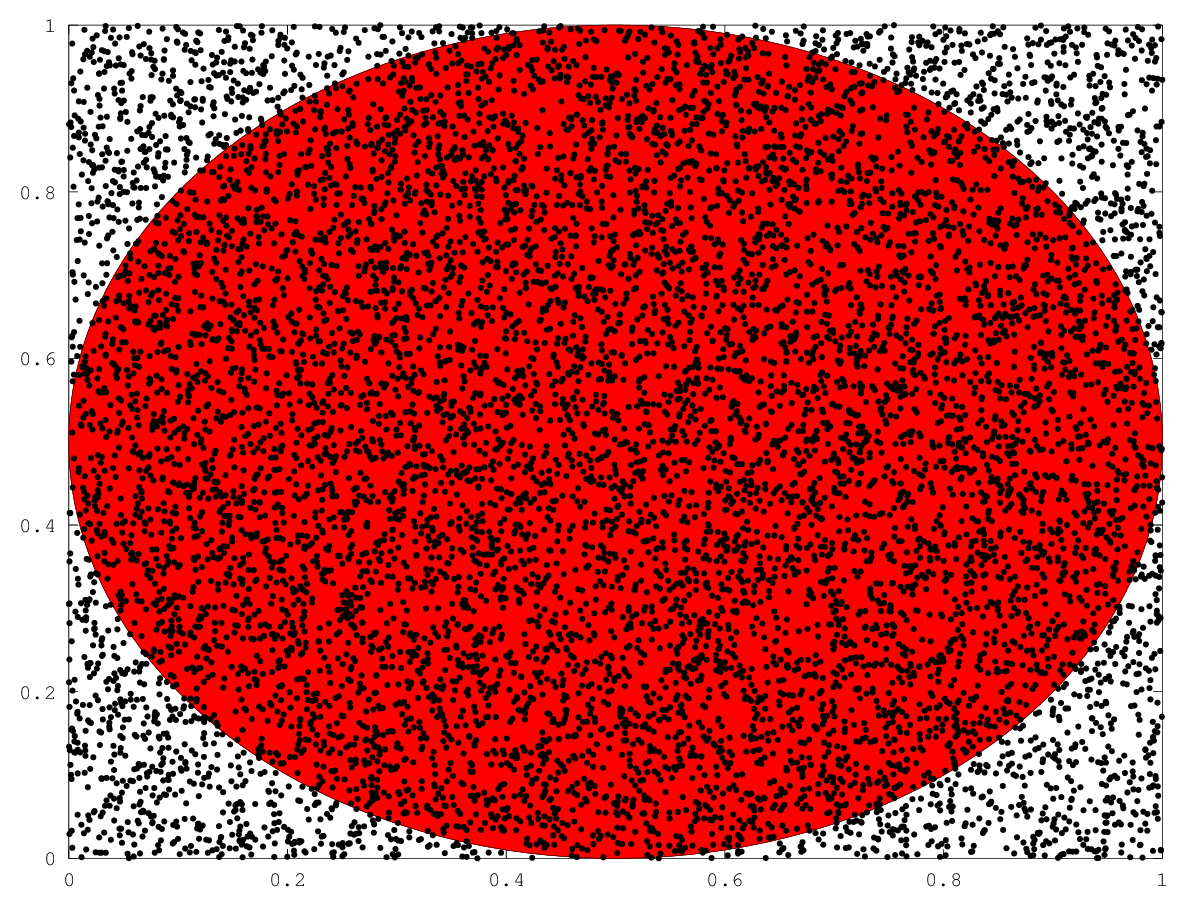
\includegraphics[scale=0.4]{num1_9_4/b.png}
			\end{figure}
		\newpage
		\item
			Test für $r(\phi)=0.4 + 0.1 \sin(8\phi)$:
			\lstinputlisting[language=matlab]{num1_9_4/c.m}
			\begin{table}[h]
				\centering
				\caption{Ergebnisse}
				\begin{tabular}{c|r}
					$n$ & $F$ aus Monte-Carlo \\ \hline
					50 & 0.52400 \\
					500 & 0.52200 \\
					5000 & 0.51712 \\
					10000 & 0.51745
				\end{tabular}
			\end{table}
			\begin{figure}[h]
				\centering
				\caption{Exemplarische Verteilung der Zufallszahlen für $n=10000$}
				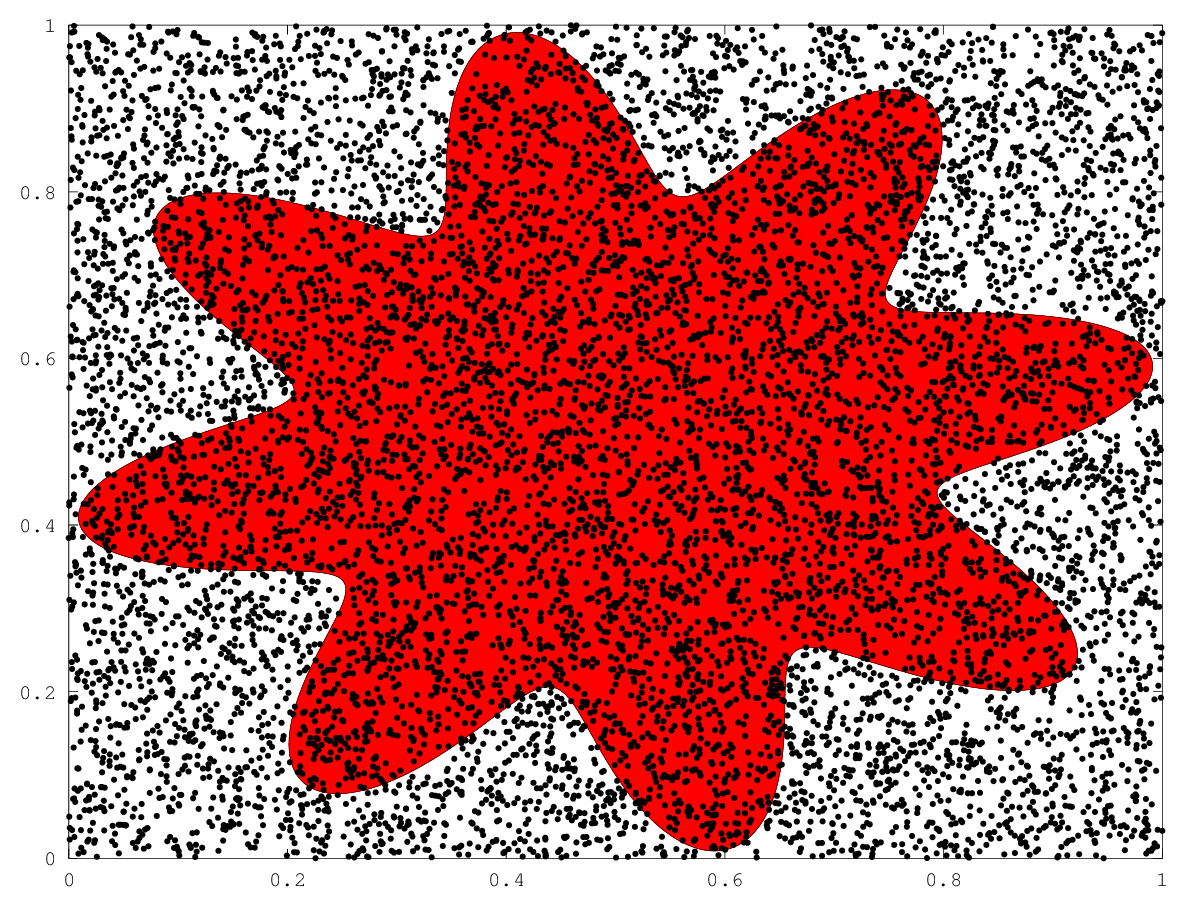
\includegraphics[scale=0.4]{num1_9_4/c.png}
			\end{figure}
						
	\end{enumerate}
\end{aufgabe}
\end{document}
